\documentclass[a4paper]{article}
\let\svthefootnote\thefootnote
\usepackage[margin=25mm]{geometry}
\usepackage{amsmath}
\usepackage{amsfonts}
\usepackage{amssymb}
\usepackage{graphicx}
\pagenumbering{gobble}
\usepackage{amssymb} %for set symbols
\usepackage{verbatim}
\usepackage{amsmath}
\usepackage{listings}
\usepackage{array}
\usepackage[utf8]{inputenc}
\usepackage{color}
\usepackage{listings}

\usepackage{float}
\usepackage[section]{placeins}
\immediate\write18{texcount -tex -sum  \jobname.tex > \jobname.wordcount.tex}

\usepackage{color}
\usepackage{hyperref}
\newcommand{\s}[1]{{\color{cyan}[S: #1]}}
\newcommand\covid{COVID-19}
\newcommand\lmi{low/middle income countries}
\newcommand\figref{Figure~\ref}

% Keywords command
\providecommand{\keywords}[1]
{
  \small	
  \textbf{\textit{Keywords---}} #1
}
\pagenumbering{arabic}
\title{EM509 Stochastic Processes Project : Random Walks}
\author{\href{https://gihan.me}{Gihan Jayatilaka}\footnote{\href{mailto:gihanjayatilaka@eng.pdn.ac.lk}{gihanjayatilaka@eng.pdn.ac.lk}} \hspace{1cm} E/14/158}
\date{09-07-2020} % Comment this line to show today's date



\begin{document}
\nocite{*}
\maketitle
\begin{abstract}
    First random walks are introduced in the order of 1D (without barriers and with barriers), 2D (without barriers and with barriers). Then Markov property is explained. The Markov property is proved for the 1D simple case and a complicated 2D case with both absorbing and reflecting barriers. Image segmentation problem is introduced from an application point of view and converted into a mathematical formulation. Random walker algorithm for image segmentation is introduced and it is proven to be a Markov process. The study is concluded by implementing the Random Walker algorithm and testing it by segmenting a set of images.
\end{abstract}

\tableofcontents


\section{Random Walks}
This section introduces random walks in an intuitive point of view and formally defines them. Later we look into different types of random walks and barrier conditions. 


Random walks refers to a kind of random processes where the current state is defined by the sum of random steps. Another way of looking at random walks is as the path traversed while making random steps.
The simplest form of Random walks are one dimensional walks along the number line ($\mathbb{Z}$) with unit steps on either direction ($\pm1$) chosen at random from an uniform distribution. More complicated random walks can be introduced starting form here by generalizing the space being traversed to 2D or N-D, allowing steps in other directions and  different distances. Furthermore, random walks can be picking steps out of different probability distributions other than uniform distributions (such as Gaussian, Poisson, etc:).
In addition to unbounded spaces listed above, random walks can happen in bounded spaces as well. The boundaries themselves can be of different shapes and have different properties such reflecting, absorbing, etc:

\subsection{Simple 1D random walk}
The simplest of random walks, 1D infinite length integer line walk can be defined as below.

\begin{figure}[h]
    \centering
    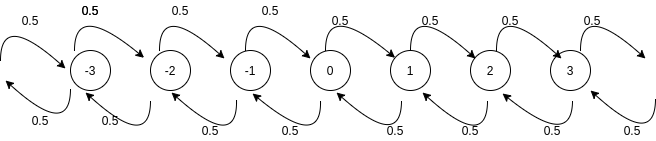
\includegraphics[width=\textwidth]{1d-unbounded.png}
    \caption{1D Simple Random walk}
    \label{fig:1d-unbounded}
\end{figure}

Assume that a particle's position at time $t$ is given by $Y_t \in \mathbb{Z}$ and $Y_0 = 0$ (the starting position is at the zero). The particle moves along the number line in integer steps $X_t$. $t \in \mathbb{Z}, t\geq0$.
$Y_t$ is given by,
$$Y_t = Y_0 + \sum_{\tau=1}^{\tau=t}X_{\tau}$$

Since $Y_0 = 0$,
$$Y_t = \sum_{\tau=1}^{\tau=t}X_{\tau}$$

$X_t$ is picked from ${-1,1}$ with equal probability.
$$X_t \sim
 \textit{U}(\{-1,+1\})$$
$$p(X_t=-1) = p(X_t=1) = 0.5$$

This gives rise to the probability distribution for $Y_{t+1}$ as,
\begin{equation}
    p(Y_{t+1}=Y_t+1)=p(Y_{t+1}=Y_t-1)=0.5
    \label{eqn:1d-nobarrier-yt}
\end{equation}

This is illustrated in \figref{eqn:1d-nobarrier-yt}
 

\subsection{2D Random walk}
We can try to extend the idea of 1D random walk to it's 2D version.

The space being walked upon ($\mathbb{Z}$ in the 1D case) is being extended to a 2D grid $\mathbb{Z}^2$ in this case. While there was only two possible steps ($\pm 1$) in 1D case, we have 4 possible steps ($\pm1$ in either dimension) in the 2D case. We can define the random process as,
$$X_t \in \{(1,0), (-1,0), (0,1), (0,-1)\}$$
$$Y_0 = (0,0)$$
$$X_t \sim
 \textit{U}(\{(1,0), (-1,0), (0,1), (0,-1)\})$$
 $$\Rightarrow p(X_t)= (1,0) =  (-1,0) = (0,1) = (0,-1) = \frac{1}{4}$$

Figure \figref{fig:2d-unbounded} is an illustration of the 2D Random walk.

Application wise, most spatial information (maps, photographs) are 2D grids. Therefor, 2D random walks have a range of usecases. The example being discussed in this study (Random walker algorithm
for image segmentation) is also based on the 2D random walk. 

\begin{figure}[h]
    \centering
    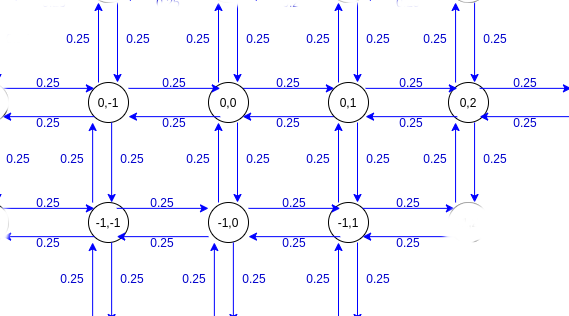
\includegraphics[width=\textwidth]{2d-unbounded.png}
    \caption{2D random walk without barriers}
    \label{fig:2d-unbounded}
\end{figure}

\subsection{Random walks with barriers}

\subsubsection{1D case}
In reality, we dont have infinitely large spaces for random walks. Therefore, we cannot practically talk about $Y_t \in \mathbb{Z}$. Instead we have to go for bounded spaces given by,
$$Y_t \in \{y; y\in\mathbb{Z}, a\leq y \leq b\}$$

When we introduce this barrier, we have to limit the possible steps near the boundary as well. There are multiple possible behaviors for barriers such as reflecting and absorbing. 

Assume that there is an absorbing barrier at $Y_t = a$ and a reflecting barrier at $Y_t = b$. This is illustrated in \figref{fig:1d-bounded}. Their behavior can be mathematically represented as,
$$Y_t = a \Rightarrow Y_{t+1}=a$$
$$Y_t = b \Rightarrow Y_{t+1}=b-1$$

\begin{figure}[h]
    \centering
    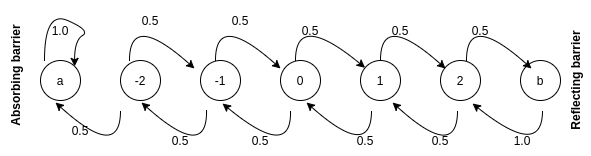
\includegraphics[width=\textwidth]{1d-bounded.png}
    \caption{1D Random walk with barriers}
    \label{fig:1d-bounded}
\end{figure}

This is achieved through limiting the steps. We started the simple random walk with only $X_t \in \{\pm1\}$. But for absorbing barrier to exist, we need to introduce another new type of step. The new set of steps would be 
$$X_t \in \{-1,0,+1\}$$. For reflecting barrier to exist, we need to allow only one step.
$$X_t \in \{-1\}$$

We introduce this new type of steps only for the absorbing barrier and reflecting barrier.,
\begin{equation*}
    X_{t+1} \in 
    \begin{cases}
    \{0\} &; Y_t = a\\
    \{-1,+1\} &; a < Y_t < b\\
    \{-1\} &; Y_t = b\\
    \end{cases}
\end{equation*}

This gives rise to new step probabilities as well.

\begin{tabular}{c|c|c}
\hline
     $Y_t$ & $p(X_{t+1})$ & $p(Y_{t+1})$ \\
\hline
     $a$&  $p(X_{t+1} = 0)=1.0$ & $p(Y_{t+1}=a)=1.0$\\
     $(a,b)$&  $p(X_{t+1} = -1)=p(X_{t+1} = 1)=0.5$ & $p(Y_{t+1}=Y_t-1)=p(Y_{t+1}=Y_t+1)=0.5$\\
     $b$&  $p(X_{t+1} = -1)=1.0$ & $p(Y_{t+1}=b-1)=1.0$\\
\end{tabular}



\subsubsection{2D case}
Similarly, we can introduce barriers for the 2D case as well. Here, we introduce an reflecting as a rectangle with corners $(a_u,a_v),(b_u,a_v),(b_u,b_v),(a_u,b_v)$.


\begin{figure}[h]
    \centering
    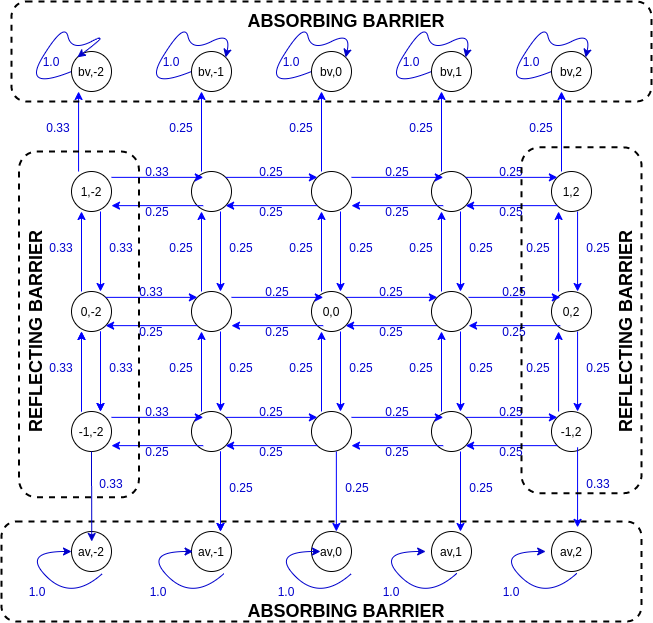
\includegraphics[width=\textwidth]{2d-bounded.png}
    \caption{2D Random walk with barriers}
    \label{fig:2d-bounded}
\end{figure}

We can define bounds for $Y_t$ as
$$Y_t \in \{y=(u,v); y=(u,v) \in \mathbb{Z}^2, a_u\leq u \leq b_u, a_v \leq v \leq b_v\}$$. 

Now we will assume that the barriers for $u$ are reflecting and the barriers for $v$ are absorbing. It is assumed that the absorbtion property takes precedence over the reflectance property. We will write the possible steps and their probabilities for this case.


\begin{equation*}
    X_{t+1} \in 
    \begin{cases}
    \{(0,0)\} &; v_t \in \{a_v,b_v\}\\
    \{(1,0)\} &; u_t = a_u \textrm{ and }a_v < v_t < b_v\}\\
    \{(-1,0)\} &; u_t = b_u \textrm{ and }a_v < v_t < b_v\}\\
    \{(-1,0), (1,0), (0,1), (0,-1)\} &; a_u < u_t < b_u  \textrm{ and }a_v < v_t < b_v\}\\
    \end{cases}
\end{equation*}

Since all these steps are equi probable (the step is picked at random from the possible set of steps) we get the following probabilities.

\begin{tabular}{|c|c|l|}
\hline
     u_t & v_t & p(X_{t+1}) \\
\hline
     a_u \leq u_t \leq b_u & v_t \in \{a_v,b_v\} & p(X_{t+1}=(0,0))=1.0 \\
     \hline
     u_t = a_u & a_v < v_t < b_v  \{a_v,b_v\} & p(X_{t+1}=(1,0))=1.0 \\
     \hline
      u_t = b_u & a_v < v_t < b_v  \{a_v,b_v\} & p(X_{t+1}=(-1,0))=1.0 \\
     \hline
     a_u < u_t < b_u & a_v < v_t < b_v & \begin{array}{l}
p(X_{t+1}=(-1,0)) =p(X_{t+1}=(1,0))\\= p(X_{t+1}=(0,-1)) = p(X_{t+1}=(0,1))\\= 0.25\end{array}\\
     
\end{tabular}

We can obtain the probabilities for $Y_{t+1}$ as\\

\begin{table}[]
    \centering
\begin{tabular}{|c|c|c|}
\hline
     u_t & v_t & p(Y_{t+1}) \\
\hline
     a_u \leq u_t \leq b_u & v_t \in \{a_v,b_v\} & p(X_{t+1}=(0,0))=1.0 \\
     \hline
     u_t = a_u & a_v < v_t < b_v  \{a_v,b_v\} & p(X_{t+1}=(1,0))=1.0 \\
     \hline
      u_t = b_u & a_v < v_t < b_v  \{a_v,b_v\} & p(X_{t+1}=(-1,0))=1.0 \\
     \hline
     
     a_u < u_t < b_u & a_v < v_t < b_v &\begin{array}{c}p(X_{t+1}=(-1,0)) = p(X_{t+1}=(1,0))\\ = p(X_{t+1}=(0,-1))= p(X_{t+1}=(0,1))\\= 0.25 \end{array}\\
     \hline
\end{tabular}
    \caption{2D Random walk with Barriers, transition probabilities}
    \label{tab:markov-2d-transition}
\end{table}

An illustration for this random walk is given in \figref{fig:2d-bounded}

\section{Markov Processes}
In this section we look at what the markov property of a random process is. Then we try to justify the markov property of the simplest random walk and a 2D random walk with barriers. This way, we establish the fact that random walks could be proven to be markov. 

\subsection{Markov Property}
Markov property refers to the memorylessness of a random process. The future states of a  random process with Markov property is dependent only on the present state. This can be mathematically formulated as below.\\
Consider a random variable $X_t$. If the conditional probability of the future states depend on all the previous states, we can write it as,
$$p(X_{t+1}) = f(X_t, X_{t-1}, X_{t-2} ....) $$ 
Here, we don't have the Markov property since we need all the previous states $X_t, X_{t-1}, X_{t-2} ....$ to predict the next state.\\
If random variable $X_t$ has the Markov property, it can be written as,
$$p(X_{t+1}) = f(X_t)$$
or using conditional probabilities as,
\begin{equation}
p(X_{t+1}|X_t, X_{t-1}, X_{t-2} ... ) = p(X_{t+1}|X_t)
\label{eqn:markov-property}
\end{equation}


\subsubsection{Markov Process}
A Markov process (also known as a Markov chain) is a random process with discrete state spaces and discrete index sets whose random variables the Markov property. 

\subsection{States of a Markov Process}
This section describes the theory behind different definitions for states in Markov processes.
\subsubsection{Communicable states}
Two states are considered communicable if there is a non zero probability of reaching either state starting from the other state.

\subsubsection{Transient states}
A state is considered transient if there is a non zero probability for a markov chain starting at that state to return back to the state.

\subsubsection{Recurrent states}
All states that are not transient are considered recurrent states.\\
\textbf{Note: } A recurrent state is not a state with a non zero probability of returning to it (which is a broader set than recurrent states). 

\subsection{Irreducibilityy of Markov Chains}
An irreducible Markov chain is a chain where any state can be reached starting from any state.\\
Markov chains with at least one absorbing state is not irreducible.


\subsection{Stationary distributions}
Intuitively, the stationary distribution is the convergent state of the Markov Chains. This can be formally defined as below.

Consider a random process with $Y_t$ and $p(Y_{t+1} | Y_t)$ taking usual meanings. Let $T$ be the transition probability martix and where 
$$T_{i,j} = p(Y_{t+1}=j | Y_{t}=i)$$ and $\pi$ being the convergent probability distribution with $$\pi_i = p(\lim_{t \to \infty} Y_{t}=i)$$

At steady state we have,
$$\pi = T\pi$$

Irreducible Markov chains have a unique $\pi$.\\
Absorbing Markov chains (Markov chains with at least one absorbing state) may have multiple $\pi$s. But all these steady states have non zero probabilities only on the absorbing states.\\


\section{Random Walks and Markov Properties}

\subsection{Simple 1D random walk as a Markov Process}
Equation \eqref{eqn:1d-nobarrier-yt} can be rewritten as,
$$p(Y_{t+1} = y | Y_t = y\pm1) =0.5 \textrm{ for all }Y_{t-1},Y_{t-2},Y_{t-3}...$$





This is of the same form as \eqref{eqn:markov-property}. $\Rightarrow$ Simple 1D random walk is a markov process.\\

The state of this markov process is $Y_t$. The state can take any value in $\mathbb{Z}$. We can graphically show the states and the transition probabilites between the states as in  \figref{fig:markov-chain-1d}.\\

Several observations we can make are,
\begin{itemize}
    \item There are infinitely many states.
    \item Every state has inward probabilities.
    \item Every state has outward probabilities.
\end{itemize}
We can draw the following conclusions,
\begin{itemize}
    \item All states (infinitely many) are recurrent states.
    
    \item Since this process has infinitely many states, there cannot exist a stationary distribution.
    \item All states are accessible from any starting state. Therefore, the markov chain is irreducible.
\end{itemize}





\subsection{2D random walk with Barriers as a markov process}

In this section we try to look into the 2D random walk with barriers (absorbing and reflecting) as a Markov process. We use the same example discusses in Table \ref{tab:markov-2d-transition}. We can clearly see how $p(Y_{t+1})$ is a function of $Y_t = (u_t,v_t)$.  This can be written as,
$$p(Y_{t+1} | Y_t) = p(Y_{t+1} | Y_t, Y_{t-1}, Y_{t-2} ...)$$
Since this equation satisfies the Markov property, 2D random walk with barriers is a Markov process.

\figref{tab:markov-2d-transition} illustrates this process. 

When considering the states in this markov chain, any walk starting at an absorbing barrier is going to be self contained. Therefore those states are recurrent.\\

Every walk staring from any other state has a non zero probability of going to the absorbing barrier and getting stuch there. Therefore, all other states are transient states.\\

An absorbing markov chain with a finite number of states is going to converge to a stationary distribution. At the stationary distribution, there will be non zero values on the absorbing states and every other state will be zero.\\

The stationary distribution is not unique because not all states are positive recurrent in this.



\section{Application : Random Walker Algorithm for Image Segmentation}

In this section we consider an application of random walks -- Random walker algorithm for image segmentation. We try to formulate the image segmentation problem as a stochastic process. We bring in the image segmentation intuition to the transition matrix of the stochastic process. Then we prove that the process is a Markov chain. Finally, we look into the results obtained by the algorithm.

\subsection{Images}

Images are 2D grids of pixels. Individual pixels may be monochromatic (scalars), RGB (3 dimensional vectors) or multi/hyper spectral (higher dimensional vectors. For this section, we consider RGB images. Assuming that they are of height $H$ and width $W$, we can represent the image as $I_{H\times W\times 3}$.

\subsection{Segmentation}

Segmentation is the process of splitting image pixels into different classes for a particular objective (e.g. segmenting by colour, background-foreground, texture, etc:.) Segmentation can also be considered as a pixelwise classification problem.\\
Usually, segments consist of blobs of connected pixels. Figure \ref{fig:img-segmentation-example} shows a practical case of image segmentation. Different colour shades are applied over different segments.\\

\begin{figure}[h]
    \centering
    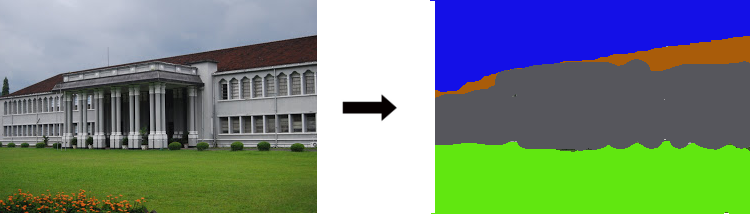
\includegraphics[width=0.5\textwidth]{image-segmentation.png}
    \caption{Image segmentation example. The image is divided into multiple segments and labelled them by colours}
    \label{fig:img-segmentation-example}
\end{figure}

\subsection{Mathematical formulation of image segmentation}
We define a function $f$ for image segmentation. The input images are considered to be $I_{H\times W\times 3}$ and the output is considered to be a $S_{H\times W}$ matrix with integers denoting the segment label for individual pixel.

$$f : I_{H\times W\times 3} \longrightarrow S_{H\times W}$$

$f$ is dependent on a distance measure $g$ between the pixels. In this study, we use the second norm of the difference between colour vectors as the distance. 

$$g(I_{(u_i,v_i)},I_{(u_j,v_j)}) = \|I(u_i,v_i) - I(u_j,v_j) \| $$


\subsection{Random Walker Algorithm}

In order to solve formulated problem, we introduce an algorithm based on random walks. The algorithm design is as following,
\begin{itemize}
    \item The image is considered to be a 2D grid with reflecting barriers on the edges.
    \item We require the used to input $N_0$ (an arbitrary number) pixel's segment labels. These pixels should include at least one pixel from every segment. This is shown in \figref{fig:rw1}. The pixles marked 1, 2 are the user inputs. Rest of the pixels are to be segmented.
    \item Since there are $H\times W$ pixels in the image and only $N_0$ are labelled, we have $HW - N_0$ pixles to segment.
\end{itemize}

How the algorithm solves the problem is as following.
\begin{enumerate}
    \item Initialize $N_1 = HW - N_0$ random walkers from the unlabelled pixels. An example is shown in \figref{fig:rw2}. We are initializing random walkers on top left and right.
    \item Let the random walkers traverse the grid until they land on one of the originally labelled pixels. This is shown in \figref{fig:rw3}.
    \item The starting pixel of the random walker gets the label of the labelled pixel it first reach.
\end{enumerate}

We index the image with $(0,0)$ in the top left. $(u,v)$ is situated $u$ pixels down and $v$ pixels right from the origin. The bottom right pixel is indexed as $(H-1,W-1)$.

The random walks are carried out by a transition probability matrix. That is generated by the following steps.

Consider a random walker at state $Y_t = (u_t,v_t)$.

\begin{table}[]
    \centering

\begin{tabular}{c|c|c}
     \hline
     $u_t$ &  $v_t$ & $X_{t+1}$ \\
     \hline
     (u_t,v_t)\in N _0 & & \{(0,0)\}\\
     \hline
     0 & 0 & \{(1,0),(0,1)\}\\
     0 & W-1 & \{(1,0),(0,-1)\}\\
     H-1 & 0 & \{(-1,0),(0,1)\}\\
     H-1 & W-1 & \{(-1,0),(0,-1)\}\\
     \hline
     0 & 1 \leq v_t \leq W-2 & \{(1,0),(0,1),(0,-1)\}\\
      H-1 & 1 \leq v_t \leq W-2 & \{(-1,0),(0,1),(0,-1)\}\\
      1\leq u_t \leq H-2 & 0 & \{(-1,0),(1,0),(0,1)\}\\
      1\leq u_t \leq H-2 & W-1 & \{(-1,0),(1,0),(0,-1)\}\\
     \hline
     1 \leq u_t \leq H-2 & 1 \leq v_t \leq W-2 & \{(-1,0),(1,0),(0,-1),(0,1)\}\\
\end{tabular}
    \caption{Possible steps for random walkers}
    \label{tab:steps-for-random-walkers}
\end{table}

Please note that the first $N_0$ points are considered to be absorbing states.

In order to assign the probabilities $p(X_{t+1})$, we consider the difference of the pixels. Consider the case where $Y_t = (u_t,v_t)$ and $X_{t+1} | Y_{t}$ can take $M$ values. The probability of the random walker picking a particular realization of $X_{t+1}$ is given by,

\begin{equation}
p(X_{t+1} = x_i) = \frac{e^{-|I(Y_t) - I(Y_t + x_i)|^2}} { \sum_{x_j \in X_{t+1}|Y_t } e^{-|I(Y_t) - I(Y_t + x_j)|^2} }
\label{eqn:xt-equation-walker}
\end{equation}

Please note that the symbol $X_{t+1}$ is used for the random variable and $X_{t+1}|Y_t$ is used to denote the possible steps.

\begin{figure}
    \centering
    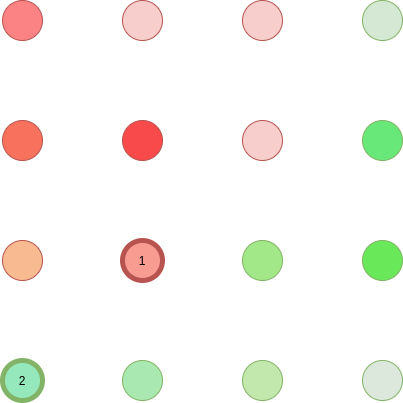
\includegraphics[width=0.5\textwidth]{rw-1.png}
    \caption{The iunitialization of the Random Walker Algorithm. Individual pixels have colours. Two pixels have been assigned segments form user input.}
    \label{fig:rw1}
\end{figure}


\begin{figure}
    \centering
    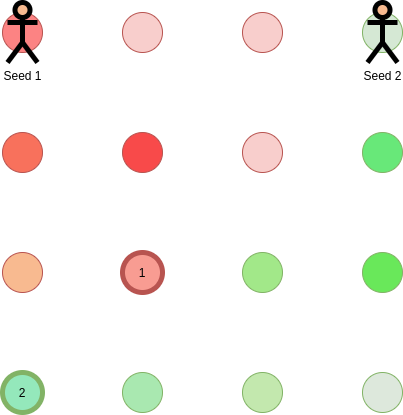
\includegraphics[width=0.5\textwidth]{rw-2.png}
    \caption{Two unlabelled pixels have been chosen to be segmented. We initalize random walks from tose pixels.}
    \label{fig:rw2}
\end{figure}

\begin{figure}
    \centering
    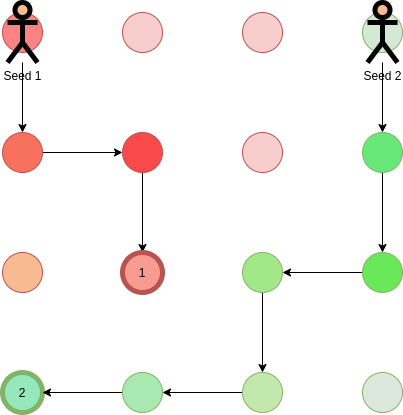
\includegraphics[width=0.5\textwidth]{rw-3.png}
    \caption{Random walk step. We can see there is more probability for a random walk to stay in the same colour because of how transition probabilities are assigned by colour similarity. The edges of the 2D grid acts as reflecting barriers and the random walks cannot go out of those edges. The marked pixels act as absorbing barriers.}
    \label{fig:rw3}
\end{figure}

\begin{figure}
    \centering
    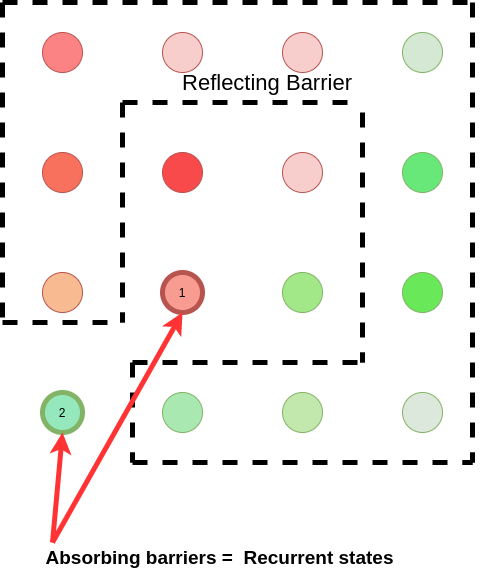
\includegraphics[width=0.5\textwidth]{rw-4.png}
    \caption{States of the Random Walker Algorithm. Absorbing states have been marked. Every other state is a transient state.}
    \label{fig:rw4}
\end{figure}
\FloatBarrier
\subsection{Markov property of the Random Walker Algorithm (including classification of states and the stationary distribution)}
We can derive an expression for $Y_{t+1}$ from \eqref{eqn:xt-equation-walker} as given in

$$p(Y_{t+1} = y_i | Y_t = y_k) = p(X_{t+1} = x_i) ; \textrm{Where }y_i = y_k + x_i$$
    
$$p(Y_{t+1} = y_i | Y_t = y_k) = \frac{e^{-|I(y_i) - I(y_k)|^2}} { \sum_{x_j \in X_{t+1}|Y_t=y_i } e^{-|I(y_i) - I(y_j)|^2} } ;\textrm{Where }y_j = y_i + x_j$$

\begin{equation}
    p(Y_{t+1} = y_i | Y_t = y_k) = f(y_i,y_k)  
    \label{yt-equation-walker}
\end{equation}

\eqref{yt-equation-walker} is in the form of Markov property. Therefore the Random Walkder Algorithm can be considered as a case of Markov Chains.

This Markov Chain has absorbing states (initially labelled pixels). Any other pixel can reach such absorbing states. Therefore, this algorithm can be categorized as an \textbf{absorbing Markov chain}.

This algorithm also has the following properties.
\begin{itemize}
    \item The absorbing states (the pixels that have a known label) are recurrent states.
    \item All other states are transient states.
    \item There are absorbing states in this system. No state can be reached from thsoe states. The Markov chain is not irreducible.
    \item There exists multiple stationary distributions. But all of them have a common property -- only absorbing states can have non zero probabilities.
\end{itemize}

The above information is clearly shown in \figref{fig:rw4}


Consider the set of stationary distributions $S$ with possible stationary distributions $\pi_i \in S$ and transition matrix $T$.\\ 
Assume that there are $M$ absorbing states. $S^M$ is the set of stationary distributions when all random walkers get absorbed to one such state. Let $\pi_j \in S^M$ be a one hot vector (only 1 element is 1, every other element is zero) with 1 on the $j^{th}$ absorbing state.\\
Every possible stationary distribution $\pi_i \in S$ can be written as a linear combinarion of $\pi_j \in S^M$








\FloatBarrier
\subsection{Implementation and results of the Random Walker Algorithm}
\subsubsection{Implementation}
We implement the proposed algorithm using the following technologies as given in table below.\\
\begin{tabular}{|l|l|}
\hline
     Python & for scripting \\
     Numpy & for numerical calculations\\
     OpenCV & for image handling\\
\hline
\end{tabular}

\\The code in given in Appendix.

\subsubsection{Experiments and Results}

As an example for the performance of the implemented algorithm, we show the results from \figref{fig:img-segmentation-example} as the ground truth.\\

The process is shown  in \figref{fig:ran-20}. We start with 4 segments and manually mark 20 pixels for each segment (left). Then we initalize random walker algorithm. The segments given by random walkers according to the stationary distribution they converge to is given in \figref{fig:ran-20}. 

It can be seen that the algorithm is not good at segmenting such structures (with fine features).

Then we look at a simpler image of an aquarium for segmentation in \figref{fig:seg-aquarium}. The results obtained are adequate.
\begin{figure}
    \centering
    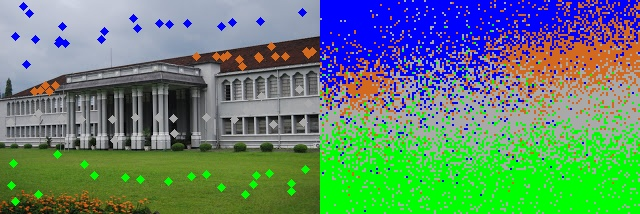
\includegraphics[width=\textwidth]{seg-20.jpg}
    \caption{Performance of the Random Walker Algorithm on the Pradeniya Photograph}
    \label{fig:ran-20}
\end{figure}

\begin{figure}
    \centering
    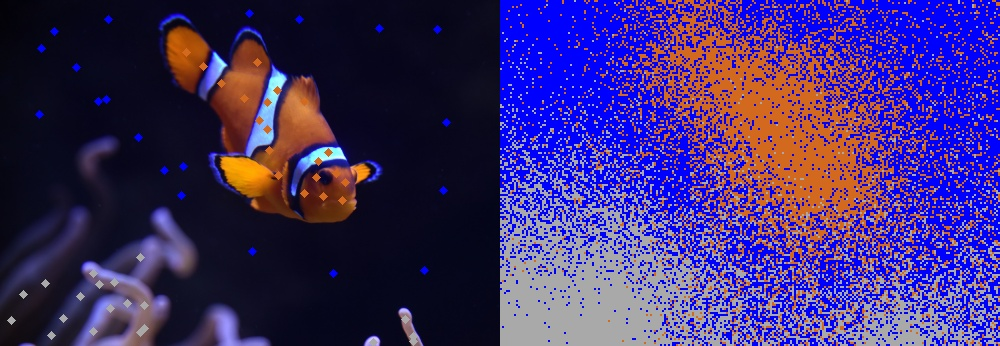
\includegraphics[width=\textwidth]{seg-fish.jpg}
    \caption{Performance of the Random Walker Algorithm on the Aquarium}
    \label{fig:seg-aquarium}
\end{figure}




\FloatBarrier
\bibliographystyle{unsrt}
\bibliography{main}
% Word count
\section{Appendix}



% Default fixed font does not support bold face
\DeclareFixedFont{\ttb}{T1}{txtt}{bx}{n}{12} % for bold
\DeclareFixedFont{\ttm}{T1}{txtt}{m}{n}{12}  % for normal

% Custom colors

\definecolor{deepblue}{rgb}{0,0,0.5}
\definecolor{deepred}{rgb}{0.6,0,0}
\definecolor{deepgreen}{rgb}{0,0.5,0}


% Python style for highlighting
\newcommand\pythonstyle{\lstset{
language=Python,
basicstyle=\ttm,
otherkeywords={self},             % Add keywords here
keywordstyle=\ttb\color{deepblue},
emph={MyClass,__init__},          % Custom highlighting
emphstyle=\ttb\color{deepred},    % Custom highlighting style
stringstyle=\color{deepgreen},
frame=tb,                         % Any extra options here
showstringspaces=false            % 
}}


% Python environment
\lstnewenvironment{python}[1][]
{
\pythonstyle
\lstset{#1}
}
{}

% Python for external files
\newcommand\pythonexternal[2][]{{
\pythonstyle
\lstinputlisting[#1]{#2}}}



\pythonexternal[language=Python]{algorithm.py}

\end{document}